\section{Correlation Estimation}
\subsection{Biased and unbiased ACF and correlogram spectral}
Fig.\ref{fig:1_3_a} illustrates both unbiased and biased estimations of autocorrelation function (ACF) and correlogram spectral with WGN, filtered WGN and noisy sinusoidal signals.  Observing the ACF diagrams, the biased and unbiased estimations are same when the lag $k$ is approximately less than 200. As the lag $k$ increases, the tendency is getting to separate in aspect of biased estimation increasing in value and the unbiased tending to zero, which verifies the Eq. \ref{proof:biase} and\ref{proof:unbiase} based on the Eq. (12)-(13) in instruction.
\begin{align}
\text{biased: } \mathbb{E}\left\{\hat r_{xx}(k)\right\} & =\frac{1}{N} \sum_{n=k+1}^{N} \mathbb{E} \left\{x(n)x^*(n-k) \right \} = \frac{N-k}{N}\ r_{xx}\label{proof:biase}\\
\text{unbiased: }\mathbb{E}\left\{\hat r_{xx}(k)\right\} & =\frac{1}{N-k} \sum_{n=k+1}^{N} \mathbb{E} \left\{x(n)x^*(n-k) \right \} = r_{xx}\label{proof:unbiase}
\end{align}
As to  correlograms of these two ACF, the biased ACF guarantees the non-negative PSD due to the positive semi-definite of ACF. However, the unbiased ACF accords to true mean of PSD, resulting to highly erratic for large lags $k$. Thus, the ACF is not positive definite and causes negative values of the PSD, which are inappropriate with theory. 
\begin{figure}[htb]
\centering
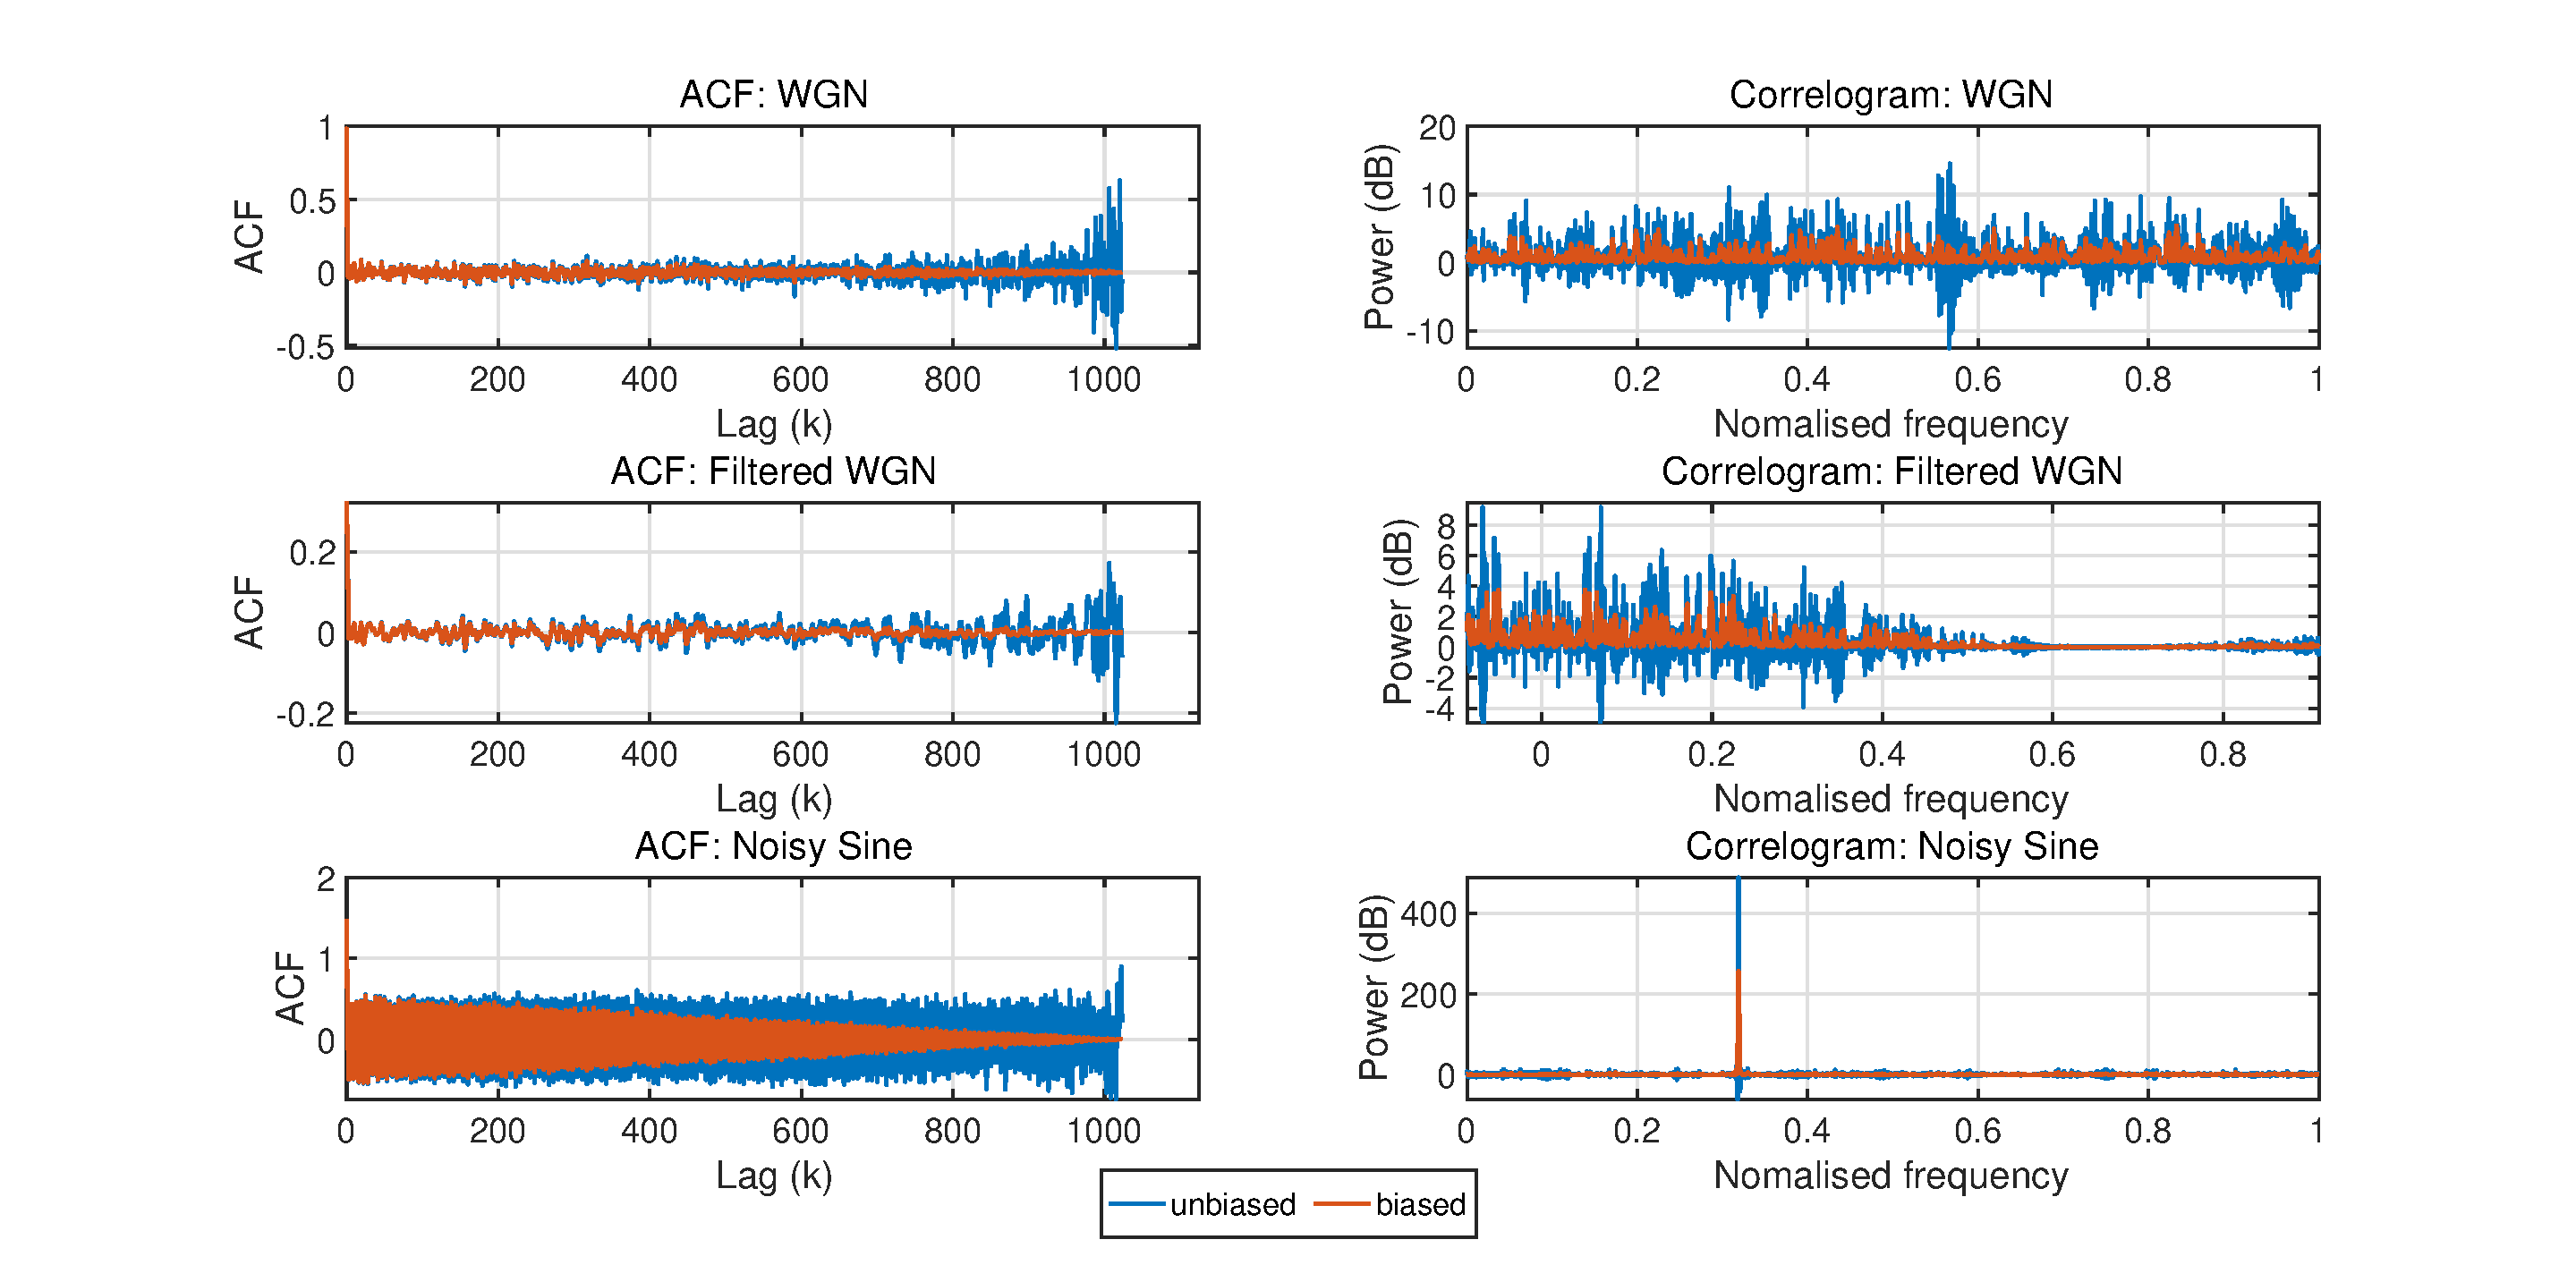
\includegraphics[width=\textwidth]{fig/13/13a.eps}
\caption{Standard and Bartlett Method of EEG Periodograms}
\label{fig:1_3_a}
\end{figure}\\
\subsection{PSD estimation with several realisations}
The PSD estimations of the signal $x(n)$ in Eq.\ref{proof:x} are plotted in Fig.\ref{fig:1_3_b} with 100 realisitions.
\begin{equation}
x(n)=sin(2\pi2n)+sin(2\pi3n)+1.5*sin(2\pi4n)+ \omega (n) \quad \omega \sim \mathcal{N} (0,1)
\label{proof:x}
\end{equation}
The mean and standard deciation of the PSD are highlighted. The signal $x(n)$ has three frequency components with $f_1=2 Hz$, $f_2=3 Hz$ and $f_3=4Hz$ which are successfully detected in the PSD. It is obvious that the variance and noise are reduced by taking mean and standard deviation. Howerver, the peak value of the PSD is to sharp. Thus, the interval between realisitions is narrow and indistinct when the PSD estimations is in magnitude scale.
\begin{figure}[htb]
     \centering
     \begin{subfigure}[b]{0.4\textwidth}
         \centering
         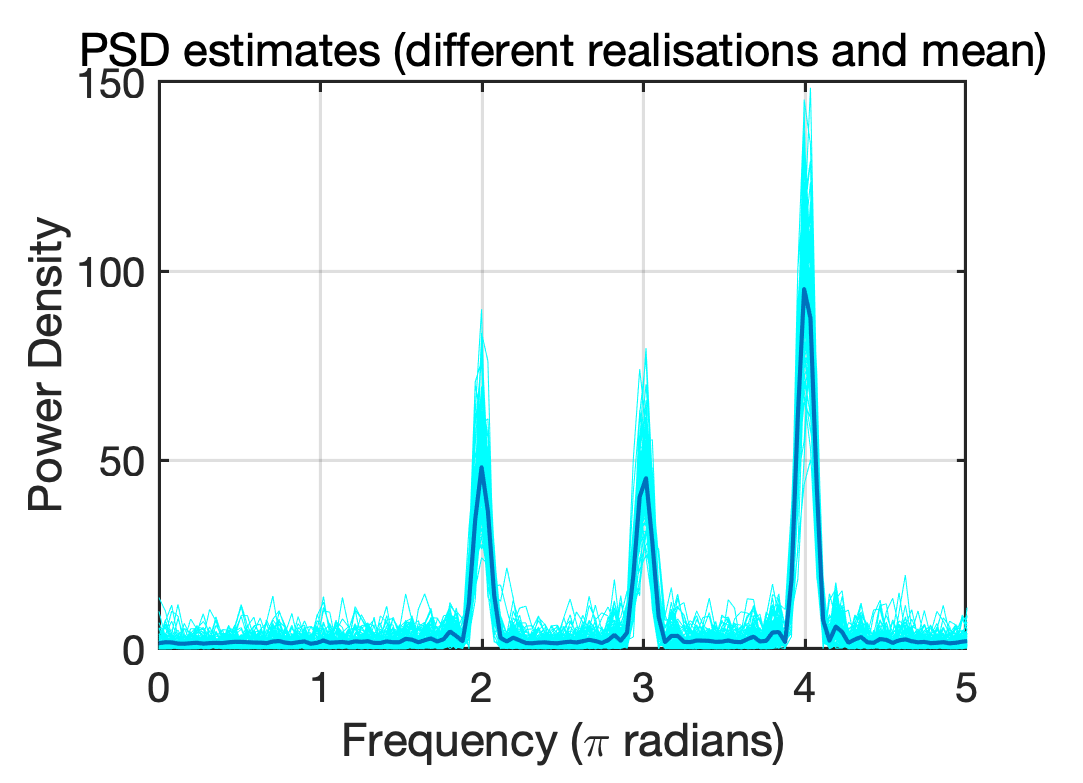
\includegraphics[width=\textwidth]{fig/13/13b1.eps}
     \end{subfigure}
     ~
     \begin{subfigure}[b]{0.4\textwidth}
         \centering
         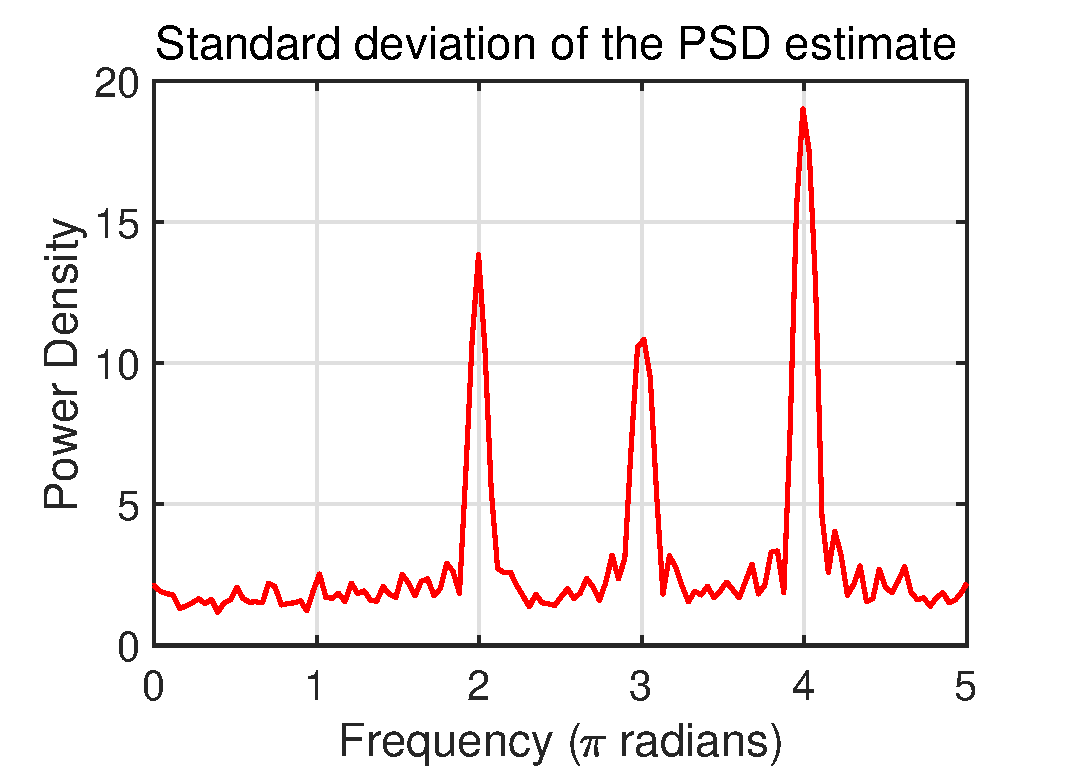
\includegraphics[width=\textwidth]{fig/13/13b2.eps}
     \end{subfigure}
        \caption{PSD estimations with mean and standard deviation}
        \label{fig:1_3_b}
\end{figure}
\subsection{PSD estimation in dB}
Repeating the process in previous section, the PSD estimations are shown in Fig.\ref{fig:1_3_c} in decibels scale. Observing the peak value of realisations, it was compressed to a large extent.  As a consequence, the amplitudes of three sinusoid signals seem to be same. Meanwhile, the noise fluctuations are significantly amplified, which increases the variance of the PSD due to the logarithm. Overall, it is an admissible and advantageous presentations to plot the PSD estimations in dB since both large and small features are visible and distinct.
\begin{figure}[htbp]
     \centering
     \begin{subfigure}[b]{0.4\textwidth}
         \centering
         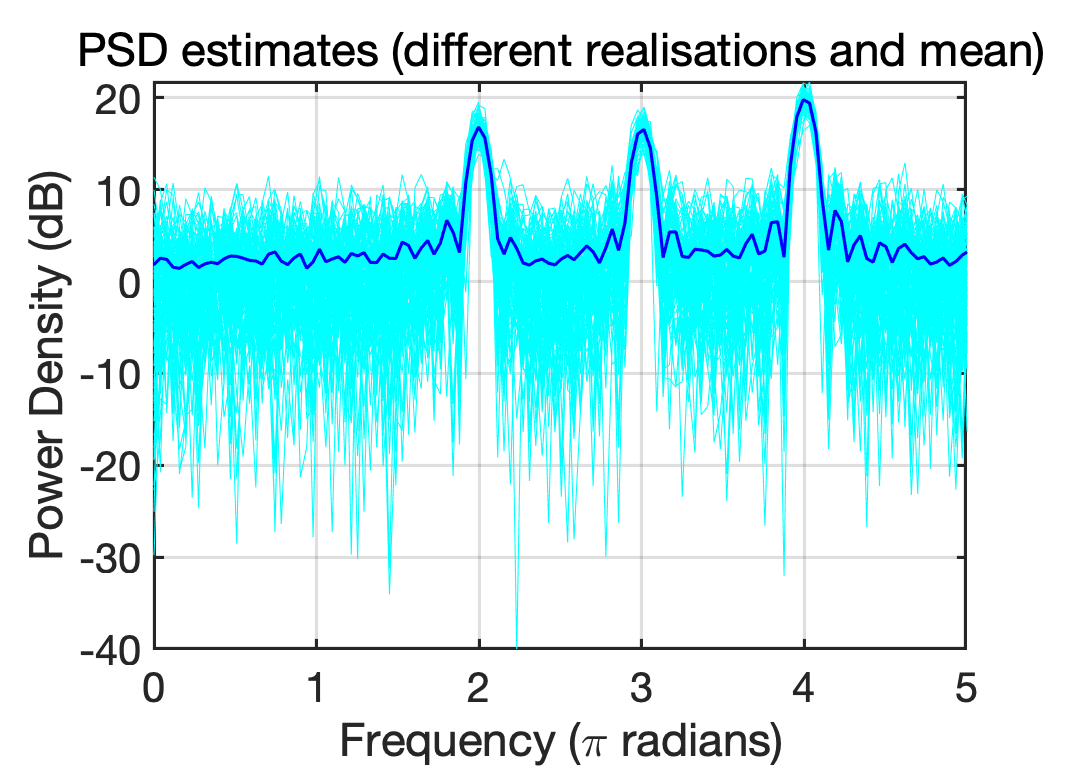
\includegraphics[width=\textwidth]{fig/13/13c1.eps}
     \end{subfigure}
     ~
     \begin{subfigure}[b]{0.4\textwidth}
         \centering
         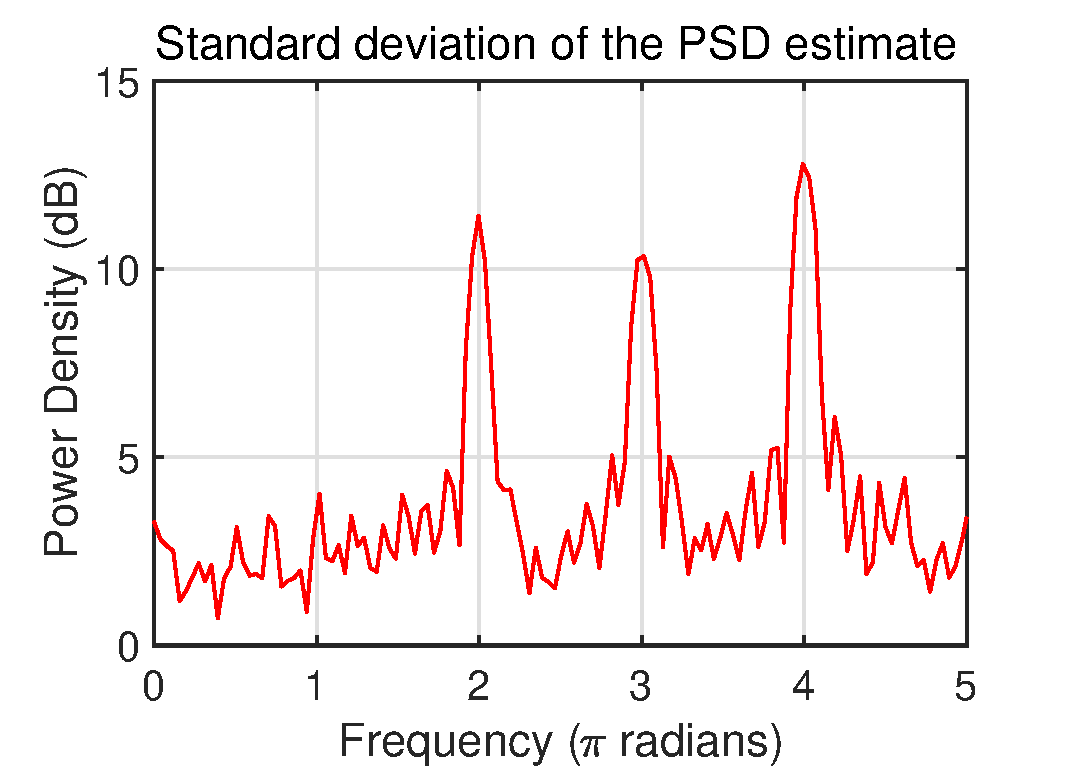
\includegraphics[width=\textwidth]{fig/13/13c2.eps}
     \end{subfigure}
        \caption{PSD estimations in dB}
        \label{fig:1_3_c}
\end{figure}
\subsection{Peak detection with window resolution}
Fig.\ref{fig:1_3_d1} depicts the periodograms of peak detection of complex-valued signal by varying the number of sample. It is obvious that the two peaks are becoming with incremental of samples ($N$), since the frequency resolution is proportional to $\frac{1}{N}$. In this experiment, the rectangular window was applied whose 3$dB$ bandwidth is defined as $0.89(\frac{2\pi}{N})$. Therefore, with two frequencies in $0.3Hz$ and $0.32Hz$ in radian, the theoretical number of samples are $N =0.89/(0.32-0.3)=44.5$. Hence, the peaks can be successfully identified when the samples are larger than 45. However, when $N$ is 40 as shown in Fig.\ref{fig:1_3_d1}, peaks are still detected which is probably caused by the sidelobes of the window.
\begin{figure}[htbp]
    \centering
    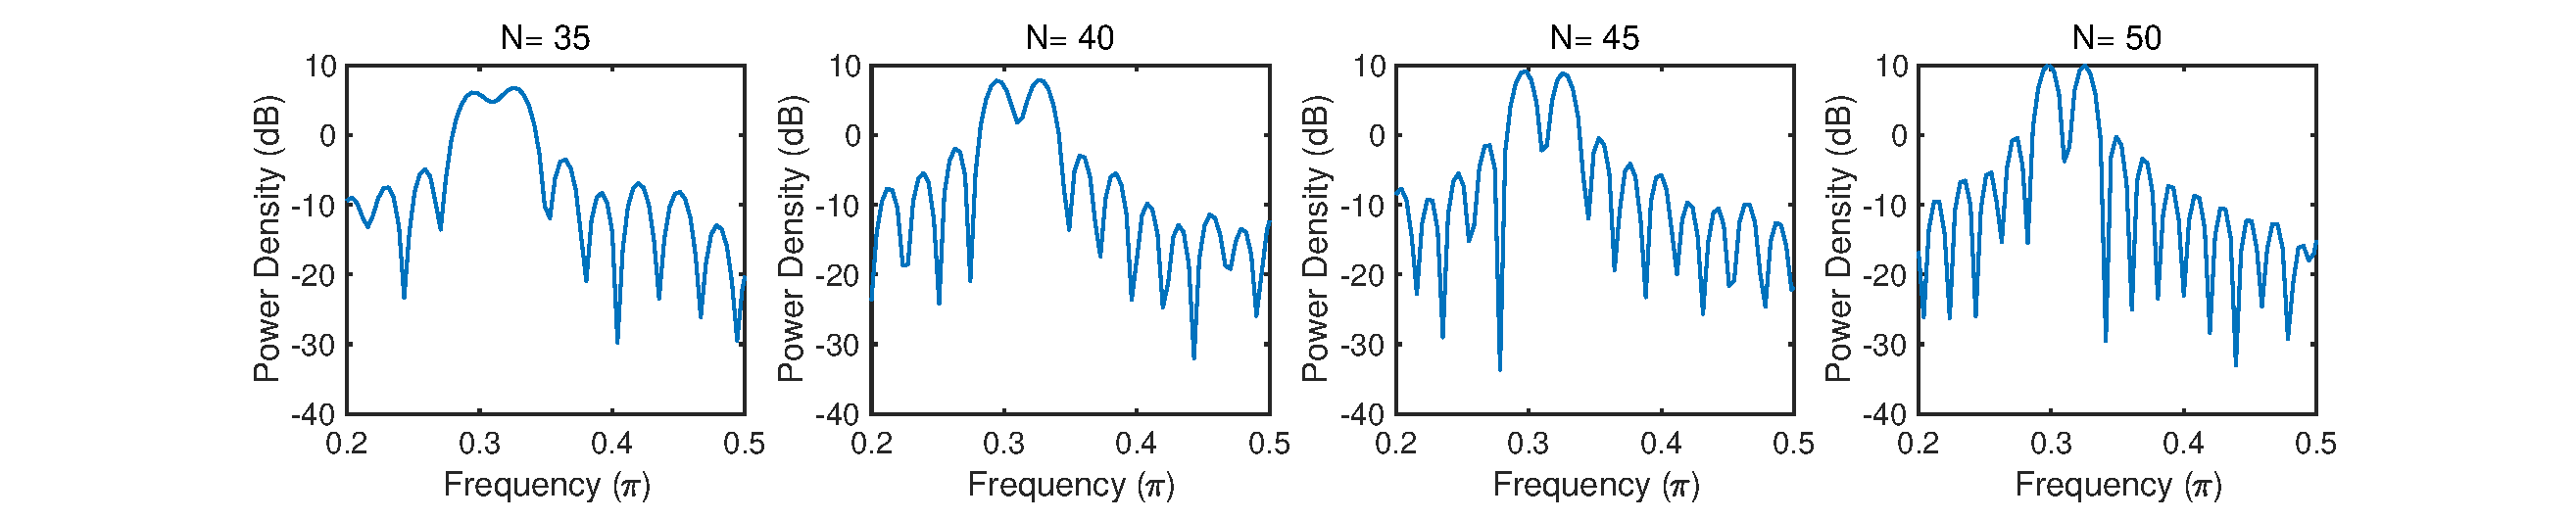
\includegraphics[width=1\textwidth]{fig/13/13d1.eps}
    \caption{Periodogram: peak detection of varying samples}
    \label{fig:1_3_d1}
\end{figure}\\
Fig.\ref{fig:1_3_d2} illustrates the peak detection with varying frequency interval from $0.32\sim0.35$. When fixing $N$ to 30, the theoretical frequency interval $\Delta f= 0.89/30 \approx 0.3$. As shown in Fig.\ref{fig:1_3_d2}, the results consist with the theory analyse where the peaks are detectable with $f2 \ge 0.33$.\\
\begin{figure}[htbp]
    \centering
    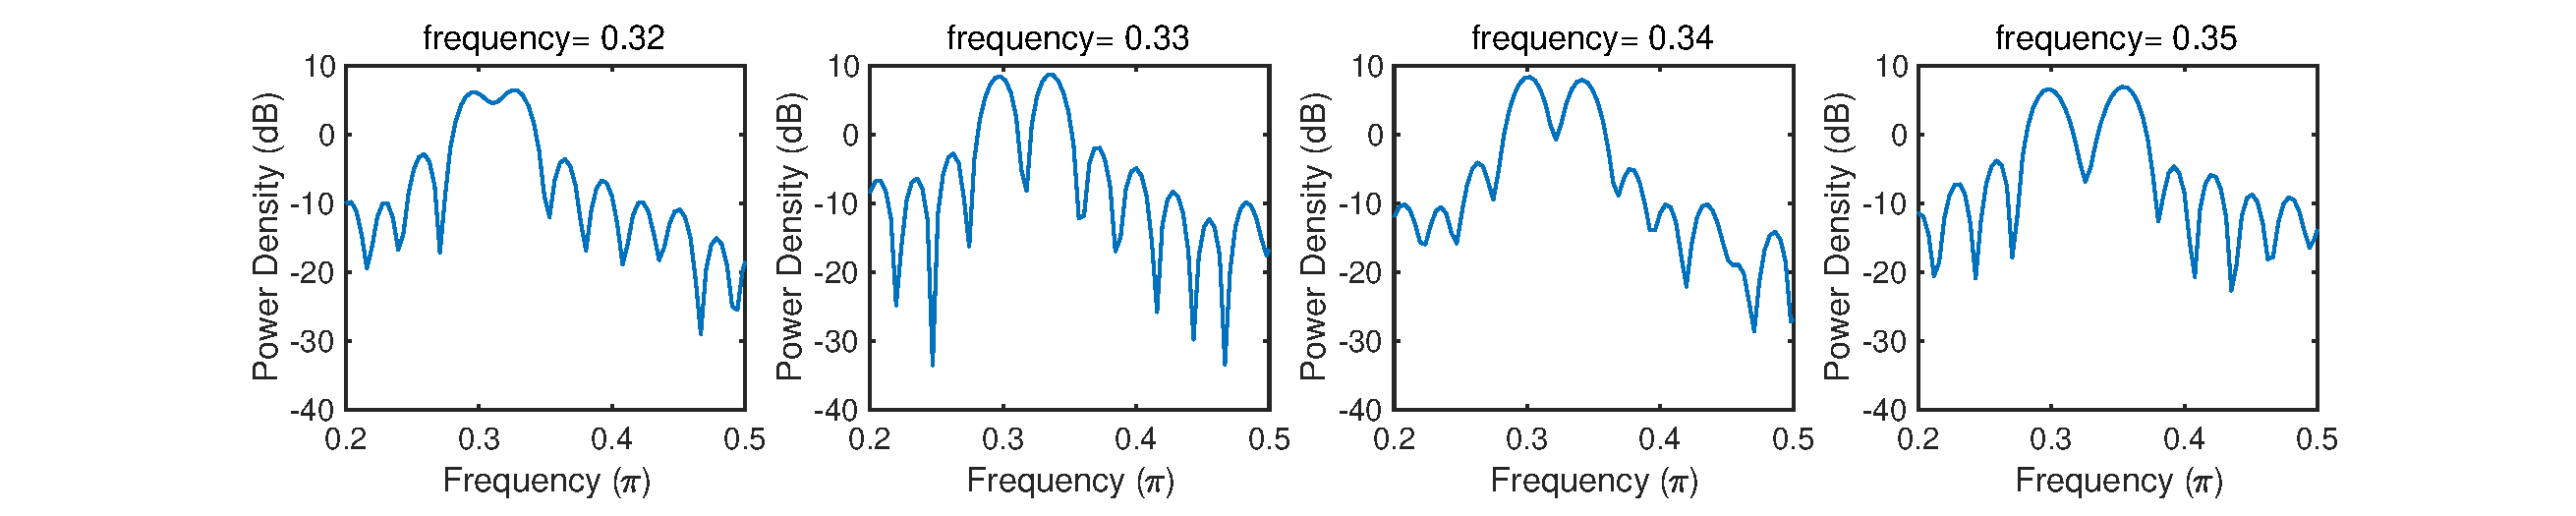
\includegraphics[width=1\textwidth]{fig/13/13d2.eps}
    \caption{Periodogram: peak detection of varying frequencies}
    \label{fig:1_3_d2}
\end{figure}
\subsection{Frequency estimation by MUSIC}
The Multiple Signal (MUSIC) algorithm is an subspace method which focusing on the eigenvectors. A complex signal with AWGN can be expressed as $\mathbf x(n)=\mathbf A \mathbf e +\mathbf w$ on vector notation. Thus, its autocorrelation matrix is calculated and decomposed into the sum of signal subspace and noise subspace, as shown below. 
\begin{equation}
\mathbb {E}(\mathbf{x x}^H)=\mathbf R_{xx}=\mathbf{EDE^H+\sigma^2I}=\mathbf{E_sD_sE^H_s+E_nD_nE^H_n}
\label{proof:Rxx}
\end{equation}
where $\mathbf{E_s=[e_1,...e_p]}$ is the eigenvectors of signal, $\mathbf{E_s=[v_{p+1},...v_M]}$ is the eigenvectors of noise and $\mathbf{D}=diag\mathbf {[A_1,...A_p,\sigma^2_{p+1}...\sigma^2_M]}$ is the eigenvalues of subspace. Due to independence between signal and noise vectors, the signal subspace and noise subspace are orthogonal, expressing in $\mathbf {e_k^Hv_i=0}$. Therefore, the MUSIC algorithm is introduced by
\begin{equation}
{\hat P_{MU}(\omega)}=\frac {1}{\sum_{i=p+1}^M \left | \mathbf{e}^H \mathbf{v}_i\right |^2}
\label{proof:music}
\end{equation}\\
In this experiment, the function \texttt{corrmtx} is used to calculated the autocorrelation matrix $\mathbf R_{xx}$ in Eq.\ref{proof:Rxx} and \texttt{pmusic} is the MUSIC function to get the peak frequency in Eq.\ref{proof:music}. Meanwhile, the $M$ is 14 and $p$ is 2 which are defined as the total dimension of the subspace and the dimension of the signal subspace respectively.\\
Fig.\ref{fig:1_3_e} depicts the estimation of the MUSIC function which is successfully detect the peaks. Comparing with the periodogram method, the MUSIC is using biased estimation and has less variance. Moreover, it can deal with less samples signal, while the periodogram method could only use long length signal due to the window resolution. However, the dimension of signal subspace $p$ need to be determined in advance, which is not practical in general cases. On the contrast, the periodogram method does not require the information of the signal.
\begin{figure}[htbp]
    \centering
    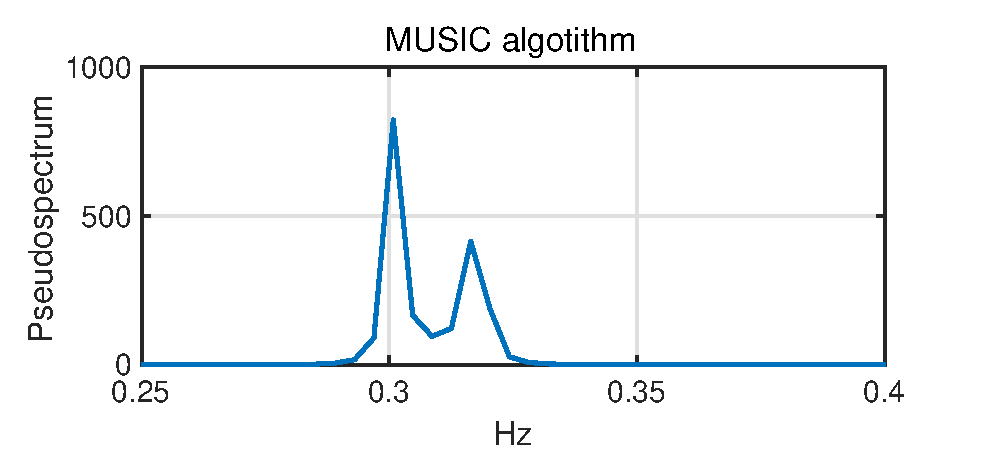
\includegraphics[width=0.6\textwidth]{fig/13/13e.eps}
    \caption{Periodogram: MUSIC algorithm}
    \label{fig:1_3_e}
\end{figure}



